% Compile with XeLaTeX, TeXLive 2013 or more recent
\documentclass{beamer}

% Base packages
\usepackage{fontspec}

\usepackage{xunicode}
\usepackage{xltxtra}

\usepackage{amsfonts}
\usepackage{amsmath}
\usepackage{longtable}
\usepackage{csquotes}
\usepackage{standalone}

\usepackage{graphicx}
\graphicspath{{./images/}}

\usepackage{tikz}
\usetikzlibrary{arrows,decorations.pathmorphing,backgrounds,positioning,fit,petri}

\usepackage{listings}
\lstset{language=C, basicstyle=\ttfamily, breaklines=true, keepspaces=true, keywordstyle=\color{blue}}

% Setup Russian hyphenation
\usepackage{polyglossia}
\setdefaultlanguage[spelling=modern]{russian} % for polyglossia
\setotherlanguage{english} % for polyglossia

% Setup fonts
\newfontfamily\russianfont{CMU Serif}
\setromanfont{CMU Serif}
\setsansfont{CMU Sans Serif}
\setmonofont{CMU Typewriter Text}

% Be able to insert hyperlinks
\usepackage{hyperref}
\hypersetup{colorlinks=true, linkcolor=black, filecolor=black, citecolor=black, urlcolor=blue , pdfauthor=Evgeny Yulyugin <yulyugin@gmail.com>, pdftitle=Параллельное программирование}
% \usepackage{url}

% Misc optional packages
\usepackage{underscore}
\usepackage{amsthm}

% A new command to mark not done places
\newcommand{\todo}[1][]{{\color{red}TODO\ #1}}

\newcommand{\abbr}{\textit{англ.}\ }

\subtitle{Курс «Параллельное программирование»}
\subject{Lecture}
\author[Евгений Юлюгин]{Евгений Юлюгин \\ \small{\href{mailto:yulyugin@gmail.com}{yulyugin@gmail.com}}}
\date{\today}
\pgfdeclareimage[height=0.5cm]{mipt-logo}{../common/mipt.png}
\logo{\pgfuseimage{mipt-logo}}

\typeout{Copyright 2014 Evgeny Yulyugin}

\usetheme{Berlin}
\setbeamertemplate{navigation symbols}{}%remove navigation symbols


\title{Параллельные архитектуры}

\begin{document}

\begin{frame}
\titlepage
\end{frame}

\section*{Обзор}

\begin{frame}{На прошлой лекции}

\begin{itemize}
    \item Общая теория параллельного программирования:
    \begin{itemize}
        \item Состояние гонки,
        \item Примитивы синхронизации,
        \item Эффективнось работы параллельного алгоритма,
        \item Закон Амдала.
    \end{itemize}
\end{itemize}

\end{frame}

\begin{frame}{На этой лекции}
\tableofcontents
\end{frame}

\section{SMP}

\begin{frame}{Симметричная мультипроцессорность}
Симметричная мультипроцессорность (\abbr Symmetric Multiprocessing, SMP) --- архитектура вычислительных систем, в которой все процессоры подключаются к общей памяти (при помощи шины или подобного устройства) симметрично и имеют к ней однородный доступ.

Так же известна как UMA (Uniform Memory Access или Uniform Memory Architecture).
\end{frame}

\begin{frame}{Симметричная мультипроцессорность}
\begin{figure}[htpb]
    \centering
    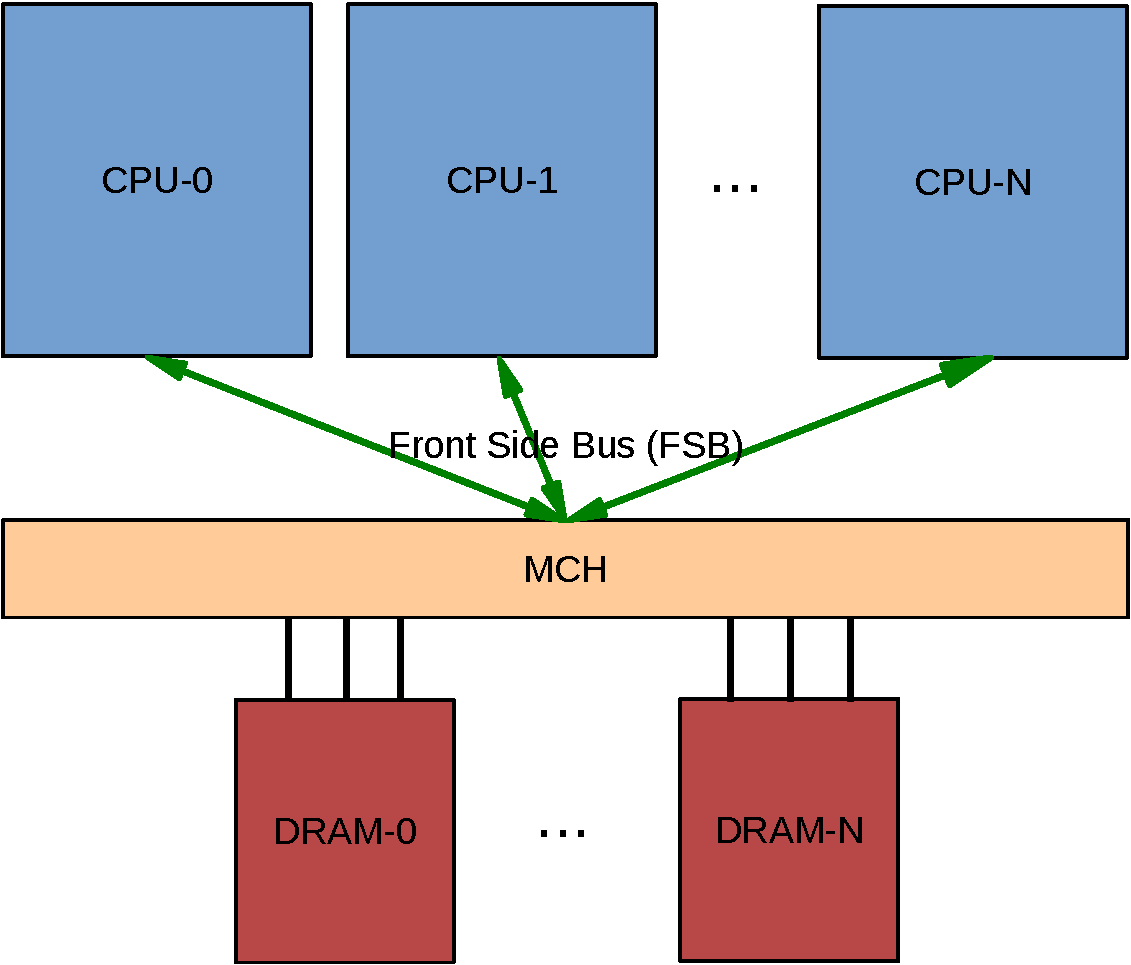
\includegraphics[width=0.7\textwidth]{SMP}
\end{figure}
\end{frame}

\begin{frame}{Преимущества}
\begin{itemize}
    \item просто и дешево масштабируется,
    \item просто программировать,
    \item выход из строя одного из процессоров выводит из строя всю систему.
\end{itemize}
\end{frame}

\begin{frame}{Недостатки}
\begin{itemize}
    \item увеличение количества процессоров $\Rightarrow$ увеличение нагрузки на шину,
    \item когерентность кэш-памяти,
    \item стоимость системы растет быстрее, чем производительность,
    \item требуется поддержка ОС.
\end{itemize}
\end{frame}

\section{MPP}

\begin{frame}{Массово-параллельная архитектура}
Массово-параллельная архитектура (\abbr Massive parallel processing, MPP) --- класс архитектур, в которых процессоры имеют доступ исключительно к локальным ресурсам. То есть память разделена физически.

Не обеспечивает встроенного механизма обмена данными между узлами. Реализовывать коммуникации и распределение должен софт.
\end{frame}

\begin{frame}{Массово-параллельная архитектура}
\begin{figure}[htpb]
    \centering
    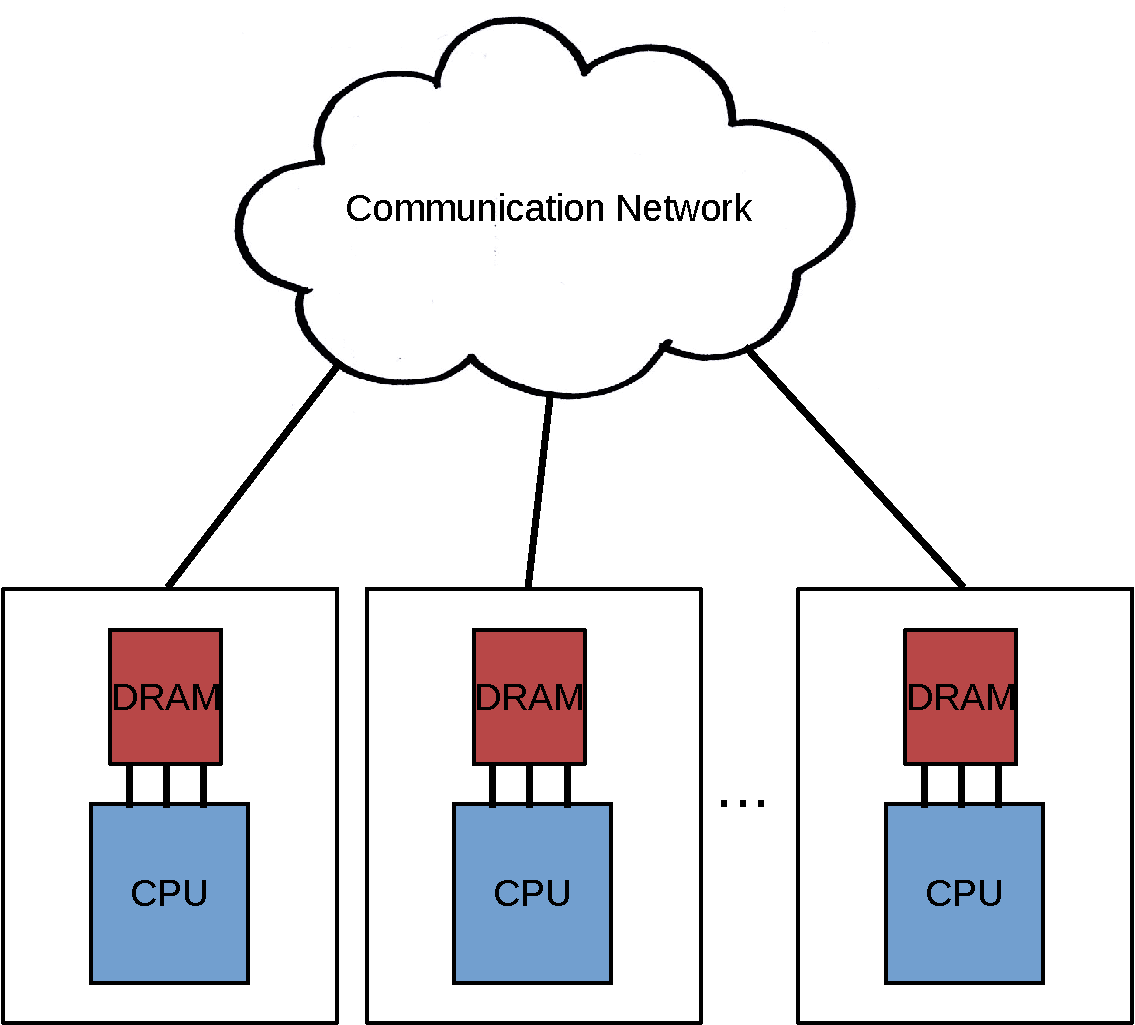
\includegraphics[width=0.65\textwidth]{MPP}
\end{figure}
\end{frame}

\begin{frame}{Преимущества и Недостатки}
Преимущества:
\begin{itemize}
    \item хорошая масштабируемость,
\end{itemize}
\vfill
Недостатки:
\begin{itemize}
    \item отсутствие общей памяти $\Rightarrow$ снижение скорости обмена данными,
    \item каждый процессор может использовать только локальную память,
    \item сложность написание ПО
\end{itemize}
\end{frame}

\section{NUMA}

\begin{frame}{Архитектура с неравномерной памятью}
NUMA (Non-Uniform Memory Access или Non-Uniform Memory Architecture) система разделяется на множественные узлы, имеющие доступ как к своей локальной памяти, так и к памяти других узлов.
\vfill
Недостатки:
\begin{itemize}
    \item доступ к удаленной памяти гораздо медленнее, чем к локальной,
    \item требует поддержки ОС.
\end{itemize}
\end{frame}

\begin{frame}{Архитектура с неравномерной памятью}
\begin{figure}[htpb]
    \centering
    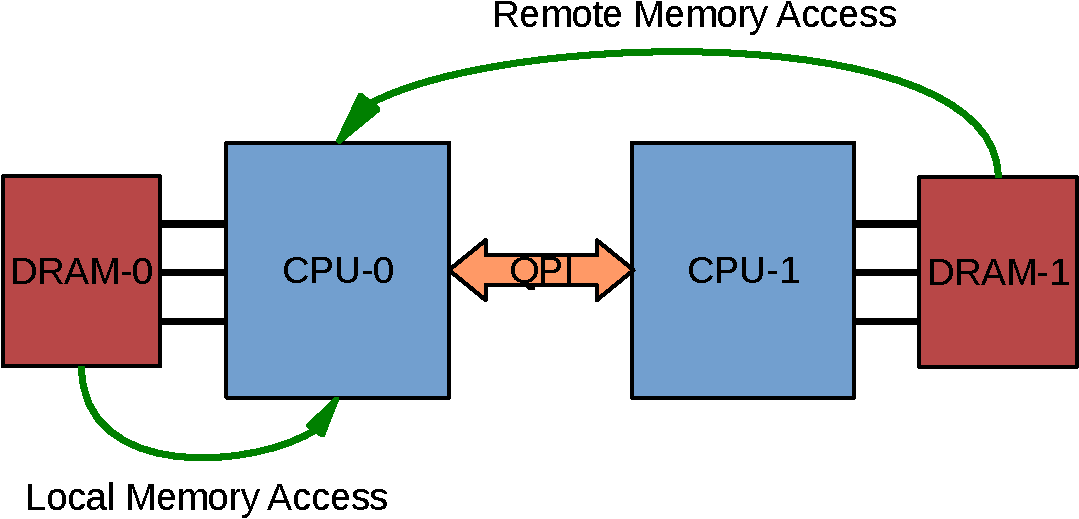
\includegraphics[width=\textwidth]{NUMA}
\end{figure}
\end{frame}

\section*{Конец}

\begin{frame}[allowframebreaks]{Рекомендуемая литература}
\begin{thebibliography}{99}
    \bibitem{} \textit{Богданов~А.В., Корхов~В.В., Мареев~В.В., Станкова~Е.Н.}
    Архитектуры и топологии многопроцессорных вычислительных систем. --- М.:
    ИНТУТ.РУ, 2004 --- 176~с. ISBN 5-9556-0018-3.
    \bibitem{} \textit{Drepper~U.} What Every Programmer Should Know About Memory
    \url{http://people.freebsd.org/~lstewart/articles/cpumemory.pdf}
\end{thebibliography}
\end{frame}

\begin{frame}{На следующей лекции}
\end{frame}

\begin{frame}

{\huge{Спасибо за внимание!}\par}

\vfill

\tiny{\textit{Замечание}: все торговые марки и логотипы, использованные в данном материале, являются собственностью их владельцев. Представленная здесь точка зрения отражает личное мнение автора, не выступающего от лица какой-либо организации.}

\end{frame}

\end{document}
